	\subsection{IntputStream类结构层次} 
	整个InputStream中大部分都在讲本地文件的读写,只有少部分关于dfs,也就是分布式文件系统。整个InputStream一条继承链和好多接口,其中FSDataInputStream实现了大部分接口。InputStream 为字节输入流,它本身为一个抽象类,基于字节的输入操作,此抽象类是表示字节输入流的所有类的超类。定义了所有输入流都具有的共同特征。必须依靠其子类实现各种功能。如图 \ref{fig:graph1} 所示
	
	\begin{figure}
		\centering
		%\includegraphics[width=3in,height=3in]{UML/inputstream/summary.jpg}
		\caption{IntputStream类结构层次}
		\label{fig:graph1}
	\end{figure}
	
	\subsection{IntputStream类结构分析} 
	Java的IO模型设计非常优秀,它使用Decorator模式,按功能划分Stream,我们可以动态装配这些Stream,以便获得您需要的功能。例如,我们需要一个具有缓冲的文件输入流,则应当组合使用FileInputStream和BufferedInputStream。另外简单数一下Java IO中的装饰模式:在IO中,具体构件角色是节点流,装饰角色是过滤流。FilterInputStream和FilterOutputStream是装饰角色,而其他派生自它们的类则是具体装饰角色。如图\ref{fig:graph2} 所示
	
	\begin{figure}
		\centering
		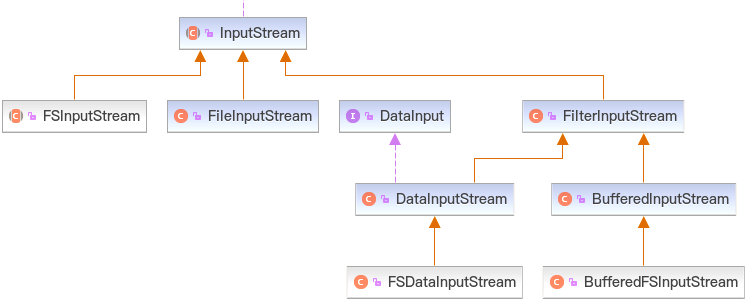
\includegraphics[width=3in,height=3in]{UML/inputstream/common-io-diagram.png}
		\caption{IntputStream部分类}
		\label{fig:graph2}
	\end{figure}
	
	\subsubsection{FSInputStream}
	FSInputStream 实现了接口 Seekable 和 PositionedReadable。提供了基本的读取一个输入流的操作,比如定位seek和读取到特定的buffer的操作read和readFully。FSInputStream在原有InputStream 基础之上添加了 getPos 方法,同时可以通过 seek 方法定位指定的偏移量处。新添加的 getPos 和 seek 方法在 FSDataInputStream 类中被使用。如图\ref{fig:graph3} 和 \ref{fig:graph4}所示
	
	\begin{figure}
		\centering
		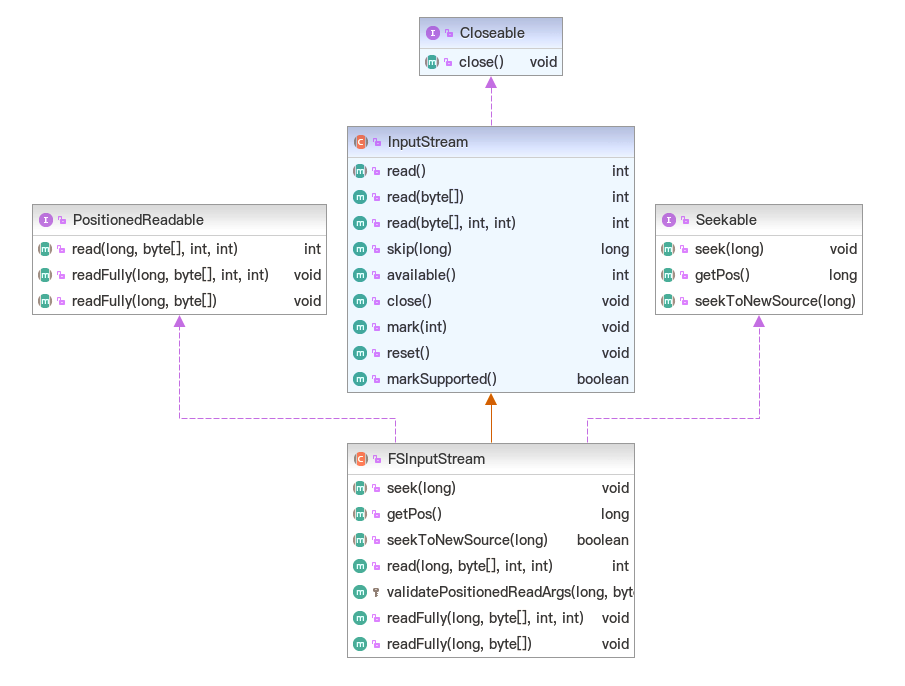
\includegraphics[width=3in,height=3in]{UML/inputstream/hdfs-fsinputstream-methods-diagram.png}
		\caption{hdfs-fsinputstream-methods-diagram}
		\label{fig:graph3}
	\end{figure}
	\begin{figure}
		\centering
		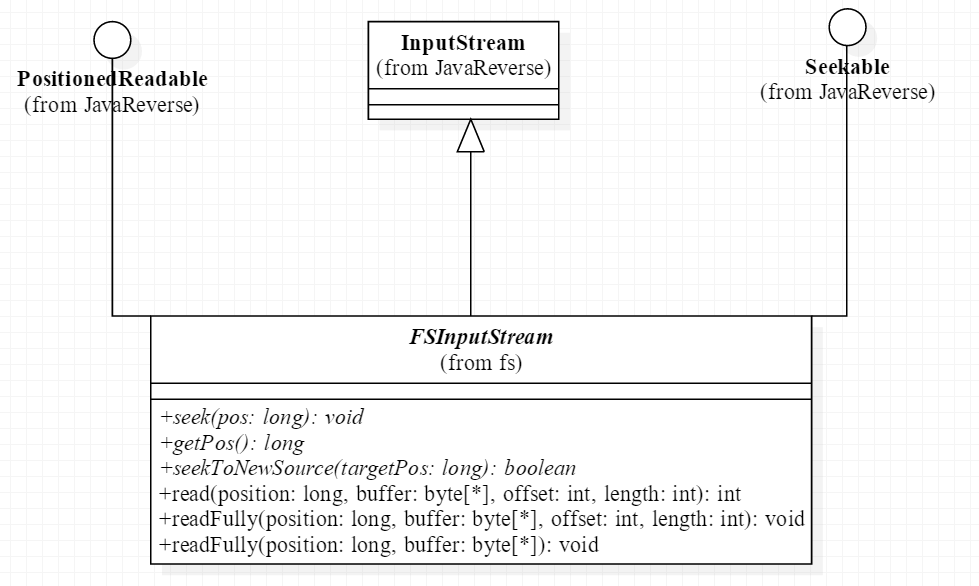
\includegraphics[width=3in,height=3in]{UML/inputstream/UML.png}
		\caption{FSInputStream类和接口}
		\label{fig:graph4}
	\end{figure}
	
	\subsubsection{PositionedReadable}
	\begin{figure}
		\centering
		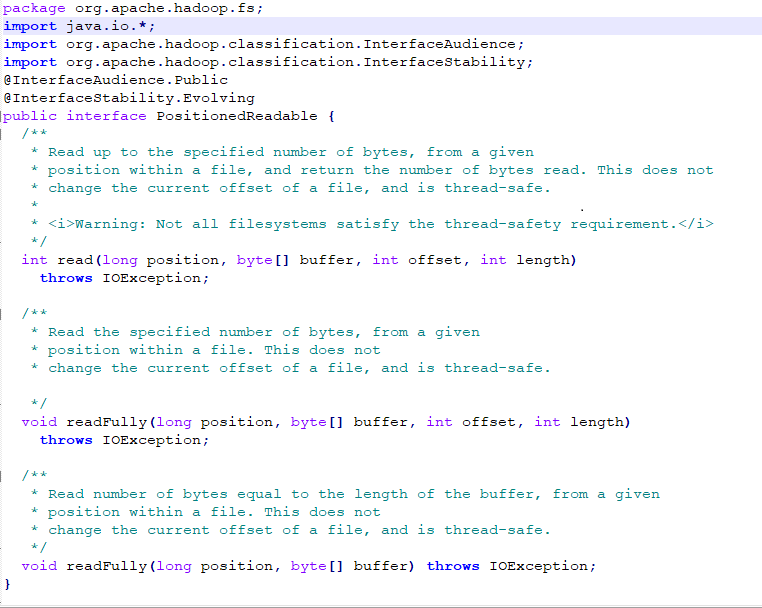
\includegraphics[width=3in,height=3in]{UML/inputstream/PositionedReadable.png}
		\caption{PositionedReadable}
		\label{fig:graph5}
	\end{figure}
	
	
	 \subsubsection{Seekable}

	\begin{figure}
		\centering
		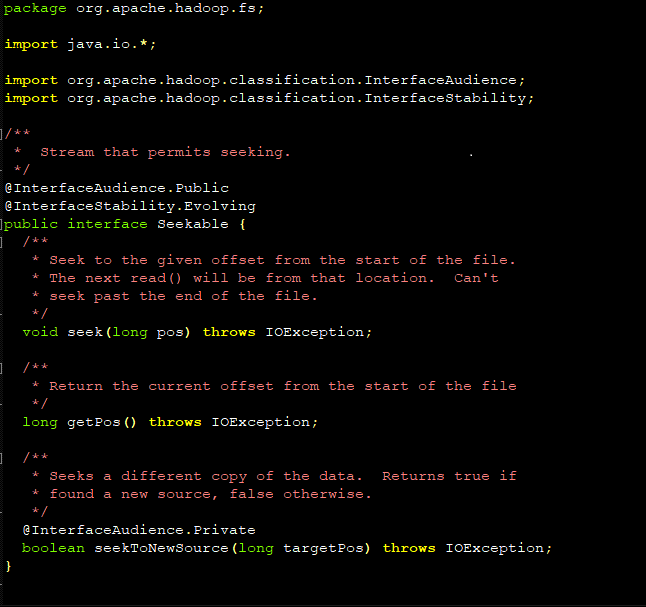
\includegraphics[width=3in,height=3in]{UML/inputstream/Seekable.png}
		\caption{Seekable}
		\label{fig:graph6}
	\end{figure}
	
	\subsection{FSInputChecker}
	FSInputChecker 提供了检测校验和的功能,主要实现了 read 方法。在 read 方法中调用了 read1方法。每当读取的数据字节数大于 maxChunkSize 时,就会调用 readChecksumChunk 方法。在readChecksumChunk 方法中,进一步调用 readChunk 抽象方法来实现真正的数据读取。读取完数据后,然后判断是否需要检验校验和,如果需要,则调用 private void verifySums(final byte b[], final int off, int read)throws ChecksumException 进行检验,如果有错,则抛出异常。abstract protected int readChunk(long pos, byte[] buf, int offset, int len,byte[] checksum) throws IOException;
	
	\begin{figure}
		\centering
		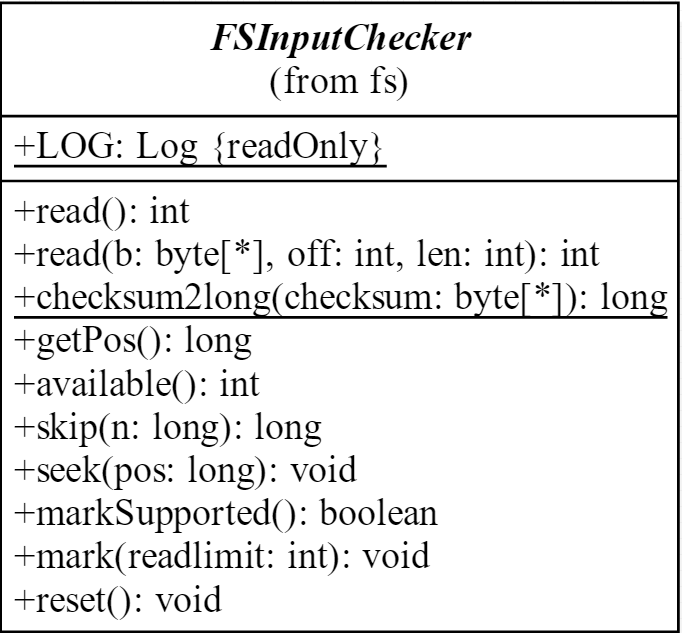
\includegraphics[width=3in,height=3in]{UML/inputstream/FSInputChecker.png}
		\caption{FSInputChecker}
		\label{fig:graph7}
	\end{figure}
	\subsection{FilterFileSystem} 
	FilterFileSystem 类包含了一个其它的文件系统的实例 fs,并将其作为基本的文件系统。FilterFileSystem 类几乎将所有重写的方法交给了其内部保存的 fs 来处理。但在交给 fs 处理之前,自己可以做一些处理,以此来实现过滤。
	\begin{figure}
		\centering
		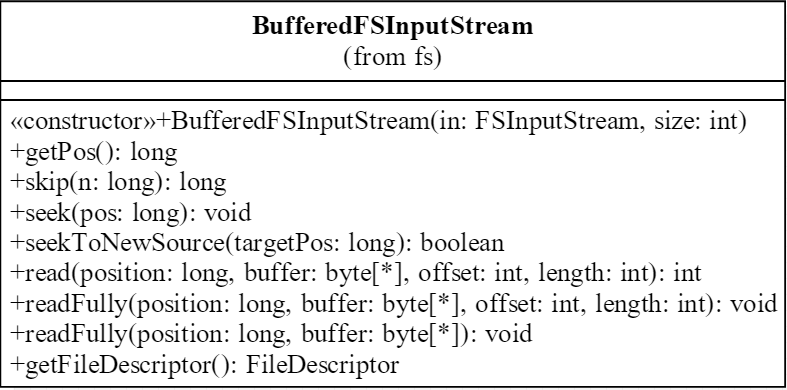
\includegraphics[width=3in,height=3in]{UML/inputstream/BufferedFSInputStream.png}
		\caption{BufferedFSInputStream}
		\label{fig:graph8}
	\end{figure}
	
	\subsection{BufferedInputStream} 
	BufferedInputStream 是缓冲输入流。它继承于FilterInputStream。
	BufferedInputStream 的作用是为另一个输入流添加一些功能,例如,提供“缓冲功能”以及支持“mark()标记”和“reset()重置方法”。
	BufferedInputStream 本质上是通过一个内部缓冲区数组实现的。例如,在新建某输入流对应的BufferedInputStream后,当我们通过read()读取输入流的数据时,BufferedInputStream会将该输入流的数据分批的填入到缓冲区中。每当缓冲区中的数据被读完之后,输入流会再次填充数据缓冲区;如此反复,直到我们读完输入流数据位置。
	
	%% end
	\endinput